\documentclass[12pt]{article}
\usepackage{sbc-template}
\usepackage{graphicx,url}
\usepackage{url}
\usepackage[brazil]{babel}
\usepackage[utf8]{inputenc}
\usepackage[T1]{fontenc}
\usepackage[normalem]{ulem}
\usepackage[hidelinks]{hyperref}

\usepackage[square,authoryear]{natbib}
\usepackage{amssymb}
\usepackage{mathalfa}
\usepackage{algorithm}
\usepackage{algpseudocode}
\usepackage[table]{xcolor}
\usepackage{array}
\usepackage{titlesec}
\usepackage{mdframed}
\usepackage{listings}

\usepackage{amsmath}
\usepackage{booktabs}

\urlstyle{same}

\newcolumntype{L}[1]{>{\raggedright\let\newline\\\arraybackslash\hspace{0pt}}m{#1}}
\newcolumntype{C}[1]{>{\centering\let\newline\\\arraybackslash\hspace{0pt}}m{#1}}
\newcolumntype{R}[1]{>{\raggedleft\let\newline\\\arraybackslash\hspace{0pt}}m{#1}}

\newcommand\Tstrut{\rule{0pt}{2.6ex}}
\newcommand\Bstrut{\rule[-0.9ex]{0pt}{0pt}}
\newcommand{\scell}[2][c]{\begin{tabular}[#1]{@{}c@{}}#2\end{tabular}}

\usepackage[nolist,nohyperlinks]{acronym}

\title{Detecção de Domínios Funcionais em Redes de Proteínas}

\author{Leandro Barcelos Ferreira\inst{1}}


\address{Universidade Federal de Uberlândia - UFU
\email{leandro.b.ferreira@ufu.br}
}



\begin{document}

	\maketitle

	\begin{resumo}
		Este trabalho modela proteínas como redes complexas para investigar se a detecção de comunidades recupera as famílias funcionais anotadas. A partir de estruturas do RCSB PDB, foram construídas redes de contato, cujas arestas ligam elementos espacialmente próximos, e uma rede de similaridade de cadeias, cujas arestas ligam cadeias com sequências semelhantes. Os modelos foram avaliados em três proteínas de teste e na proteína-alvo 6B1T. Os resultados mostram que as redes de contato recuperam a organização geométrica da estrutura, e não as famílias, enquanto a rede de similaridade recupera as famílias funcionais de forma robusta.
	\end{resumo}

	\section*{Declaração de uso de IA}

	\noindent\textbf{Modelo/versão:} Claude Sonnet 5 \\
	\textbf{Temperatura:} High

	\vspace{0.5em}
	\noindent Declaro o uso de IA no processo de desenvolvimento do código e da escrita do relatório do projeto. No código, o uso foi limitado à depuração e à solução de erros, à documentação e à otimização. No relatório, a IA foi utilizada somente para a revisão e a correção do texto.

	\section*{Declaração de colaboração}

	\noindent O projeto foi desenvolvido individualmente, sem discussões com colegas sobre a modelagem, o código ou os resultados.

	\section{Introdução}
	\label{sec_introducao}

	O objetivo deste projeto é consolidar os conceitos de modelagem de redes, medidas de centralidade e detecção de comunidades, aplicando-os à análise estrutural de proteínas. A ideia central é representar uma proteína como um grafo e verificar se a estrutura de comunidades desse grafo é capaz de identificar agrupamentos biologicamente significativos, comparando as comunidades detectadas com anotações de referência.

	O alvo do projeto é a proteína 6B1T, uma estrutura grande e multicadeia, com 25 cadeias distribuídas em 8 famílias. Como forma de validar o modelo e testar sua capacidade, ele foi primeiramente aplicado a proteínas de teste menores, a saber:

	\begin{itemize}
		\item \textbf{4HHB} --- hemoglobina humana (4 cadeias, 2 famílias: $\alpha$ e $\beta$);
		\item \textbf{1AON} --- chaperonina GroEL/GroES (21 cadeias, 2 famílias: Cpn60 e Cpn10);
		\item \textbf{6MID} --- poliproteína de flavivírus (duas famílias) em complexo com um fragmento de anticorpo (3 famílias).
	\end{itemize}

	Todo o projeto foi implementado em Python.

	\section{Obtenção e preparação dos dados}
	\label{sec_dados}

	Todos os dados vêm do RCSB PDB. Para cada proteína, foram obtidos dois tipos de informação: o arquivo de coordenadas atômicas, em formato PDB, e uma anotação das famílias funcionais de suas cadeias.

	O alvo 6B1T foi baixado como um pacote comprimido (\textit{tar.gz}), com o modelo dividido em dois arquivos PDB. As proteínas de teste foram baixadas como arquivos \textit{.pdb} individuais.

	As anotações foram feitas manualmente, a partir da descrição de cada entrada no RCSB, e salvas em um JSON que mapeia o nome da família para a lista de cadeias que pertencem a ela. Segue o exemplo para o 4HHB:

	\begin{verbatim}
# JSON: Estrutura do arquivo de anotações
{
  "Hemoglobin, alpha-type": ["A", "C"],
  "Hemoglobin, beta-type": ["B", "D"]
}
	\end{verbatim}

	A leitura dos arquivos utiliza o BioPandas, que converte o PDB em um DataFrame do pandas com uma linha por átomo. Para o pacote do 6B1T, os dois arquivos são extraídos e concatenados em um único DataFrame. Em todos os casos, consideram-se apenas os registros \textit{ATOM}.

	O DataFrame passa, então, pelo seguinte tratamento:

	\begin{enumerate}
		\item removem-se as colunas não utilizadas;
		\item descartam-se conformações alternativas (\emph{alt-loc}), mantendo-se apenas a principal, para não duplicar átomos de um mesmo resíduo;
		\item cria-se um identificador único por resíduo na forma:
			\[\text{cadeia}:\text{resíduo}+\text{inserção}\]
	\end{enumerate}

	A Tabela~\ref{tab_estruturas} resume as estruturas das proteínas utilizadas, com as contagens medidas após o processamento descrito acima.

	\begin{table}[H]
		\centering
		\caption{Estruturas utilizadas e suas contagens após o processamento.}
		\begin{tabular}{llrrrr}
			\toprule
			\textbf{PDB} & \textbf{Papel} & \textbf{Cadeias} & \textbf{Resíduos} & \textbf{Átomos} & \textbf{Famílias anotadas} \\
			\midrule
			6B1T & alvo  & 25 & 12.544 & 100.134 & 8 \\
			1AON & teste & 21 & 8.015  & 58.674  & 2 \\
			6MID & teste & 8  & 1.965  & 14.971  & 3 \\
			4HHB & teste & 4  & 574    & 4.384   & 2 \\
			\bottomrule
		\end{tabular}
		\label{tab_estruturas}
	\end{table}

	\section{Modelagem das redes}
	\label{sec_modelagem}

	Foram implementadas duas famílias de modelos: redes de contato e uma rede de similaridade de cadeias. Este capítulo apresenta as redes de contato, caracteriza sua topologia e mostra, por meio da detecção de comunidades, que elas capturam a organização geométrica da estrutura, e não as famílias. Essa análise motiva o uso da rede de similaridade de cadeias, adotada no restante do trabalho.

	\subsection{Redes de contato}
	\label{sec_contato}

	Nas redes de contato, dois nós são ligados quando a distância entre eles é inferior a um limiar, em ångströms. Elas foram escolhidas inicialmente por constituírem a modelagem mais comum na literatura de redes de proteínas \citep{vishveshwara2002, greene2003, dipaola2013}. Foram implementadas quatro variantes:

	\begin{table}[H]
		\centering
		\caption{Variantes de rede de contato implementadas.}
		\begin{tabular}{lll}
			\toprule
			\textbf{Rede} & \textbf{Nó} & \textbf{Peso} \\
			\midrule
			C$\alpha$ & átomos C$\alpha$ (um por resíduo) & opcional: inverso da distância \\
			C$\beta$ & átomos C$\beta$ (ou C$\alpha$ para glicina) & opcional: inverso da distância \\
			Resíduo & resíduo & número de contatos atômicos \\
			Cadeia & cadeia & número de contatos atômicos \\
			\bottomrule
		\end{tabular}
		\label{tab_variantes}
	\end{table}

	Nas representações por C$\alpha$ e por C$\beta$, em vez de todos os átomos, utiliza-se apenas um átomo por resíduo: carbono-$\alpha$ ou carbono-$\beta$. Nas variantes ponderadas, o inverso da distância é usado como forma de fortalecer as conexões entre átomos que estão mais próximos.

	Para as redes de resíduos e de cadeias, é gerado um grafo atômico de contato e, então, é feita uma redução para a estrutura desejada. Cada nó agrega um conjunto de átomos, e o peso das arestas representa o número de pares em contato no grafo original.

	A busca por pares próximos utiliza árvores k-d (\textit{cKDTree} do SciPy), reduzindo significativamente o custo computacional.

	\subsection{Topologia das redes de contato}
	\label{sec_topologia_contato}

	A topologia das redes de contato revela sua natureza geométrica. A Tabela~\ref{tab_topologia} resume as métricas da rede C$\alpha$ a 8 Å (valor adotado na literatura) para o alvo (6B1T) e para uma proteína de teste (1AON).

	\begin{table}[H]
		\centering
		\caption{Métricas das redes de contato (C$\alpha$, 8 Å) do alvo e de uma proteína de teste.}
		\begin{tabular}{lrr}
			\toprule
			\textbf{Métrica} & \textbf{6B1T} & \textbf{1AON} \\
			\midrule
			Nós & 12.544 & 8.015 \\
			Arestas & 66.810 & 43.334 \\
			Grau médio & 10,7 & 10,8 \\
			Grau máximo & 20 & 21 \\
			Densidade & 0,0008 & 0,0013 \\
			Clustering médio & 0,50 & 0,53 \\
			Componentes & 1 & 1 \\
			Fração no maior componente & 1,00 & 1,00 \\
			Assortatividade de grau & 0,42 & 0,31 \\
			\bottomrule
		\end{tabular}
		\label{tab_topologia}
	\end{table}

	As duas redes têm o mesmo perfil. Com o limiar de 8 Å, toda a estrutura forma um único componente conexo, com grau médio próximo de 11 e distribuição de graus em forma de sino (Figuras~\ref{fig_deg_6b1t} e~\ref{fig_deg_1aon}). Como o grau de um nó é o número de vizinhos espaciais dentro do limiar, os nós de maior grau indicam que os átomos estão em regiões mais densas, enquanto os de menor grau estão em regiões mais expostas ou nas extremidades das cadeias. O alto clustering reflete o fato de que os vizinhos de um nó tendem a ser vizinhos entre si, e a assortatividade positiva indica que nós de grau alto se conectam preferencialmente a outros nós de grau alto. A centralidade de intermediação destaca os nós situados nos caminhos entre as regiões densas do grafo (Figura~\ref{fig_betw_6b1t}), tipicamente nos pontos em que cadeias diferentes se tocam.

	\begin{figure}[H]
		\centering
		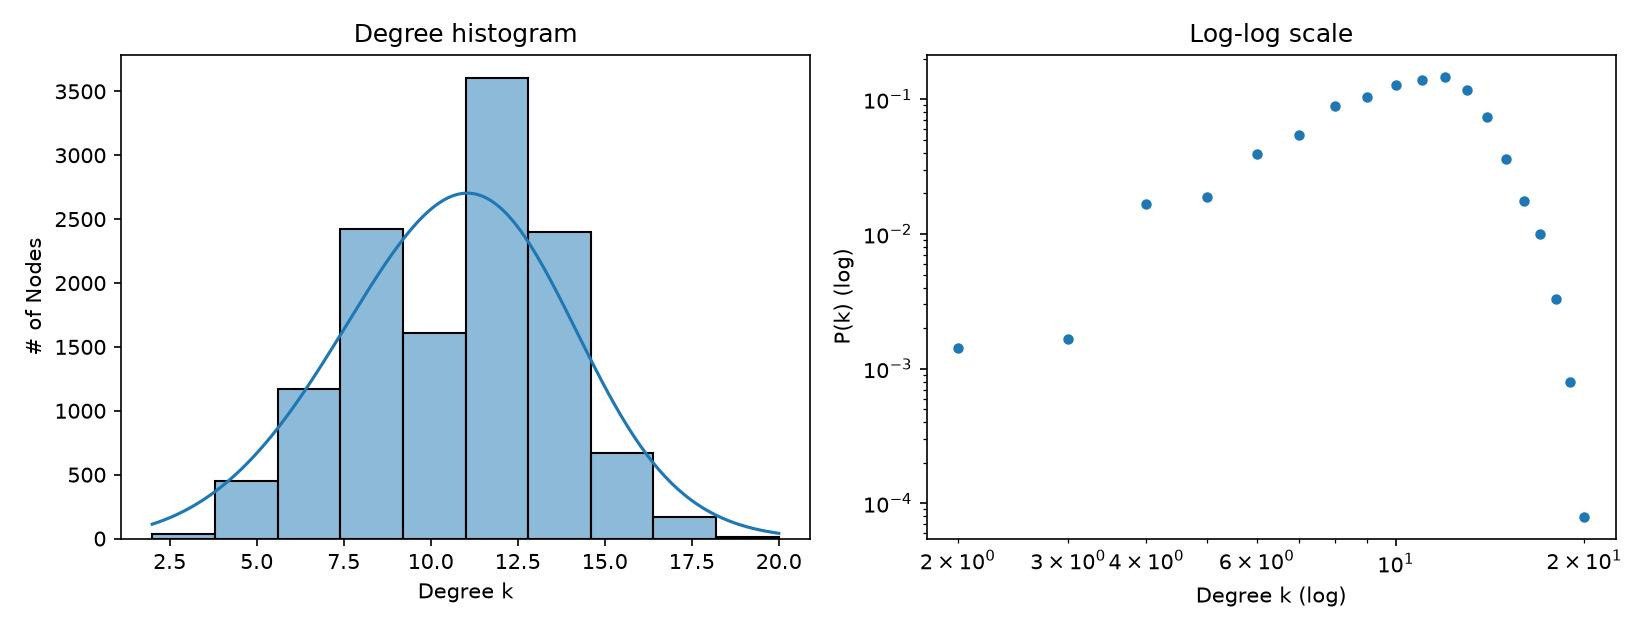
\includegraphics[width=0.95\textwidth]{figures/6B1T-contact-degree_dist.jpg}
		\caption{Distribuição de graus da rede de contato C$\alpha$ (8 Å) do 6B1T: histograma (esquerda) e escala log-log (direita).}
		\label{fig_deg_6b1t}
	\end{figure}

	\begin{figure}[H]
		\centering
		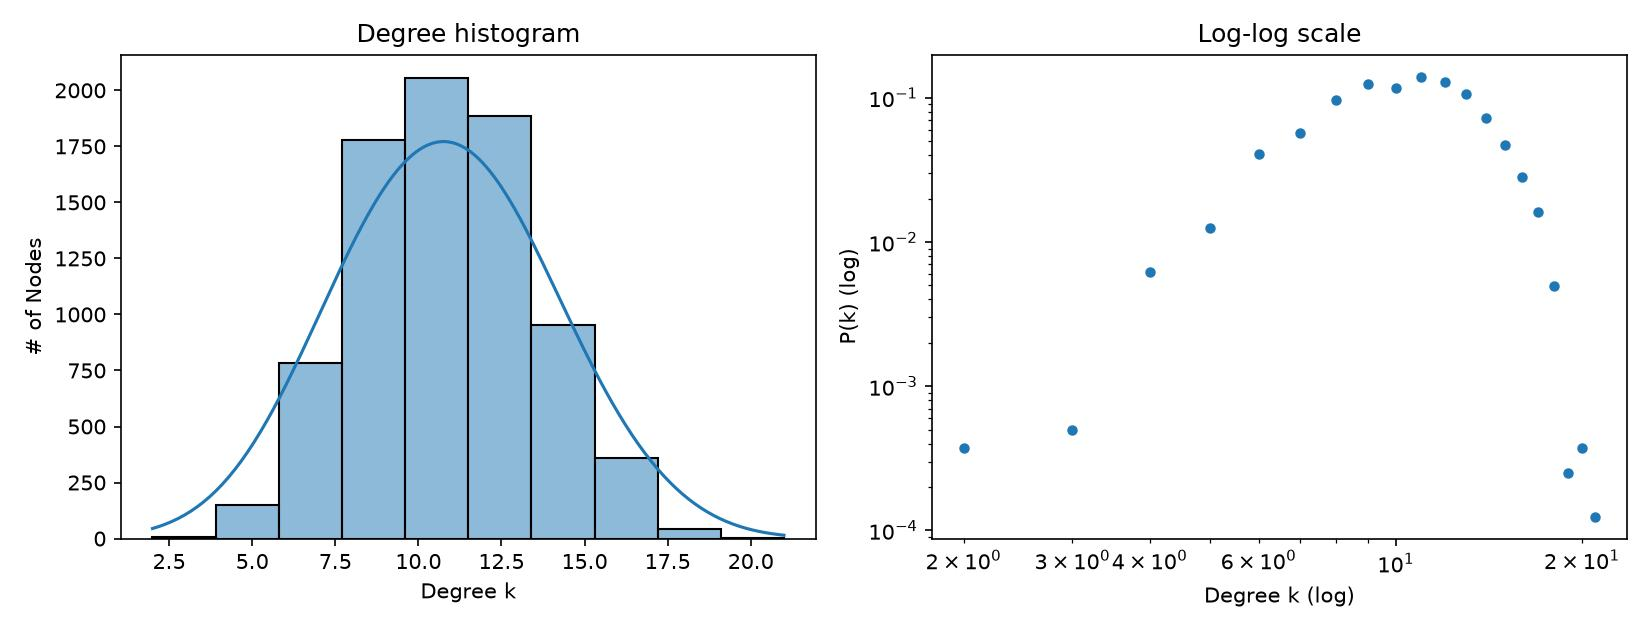
\includegraphics[width=0.95\textwidth]{figures/1AON-contact-degree_dist.jpg}
		\caption{Distribuição de graus da rede de contato C$\alpha$ (8 Å) do 1AON.}
		\label{fig_deg_1aon}
	\end{figure}

	\begin{figure}[H]
		\centering
		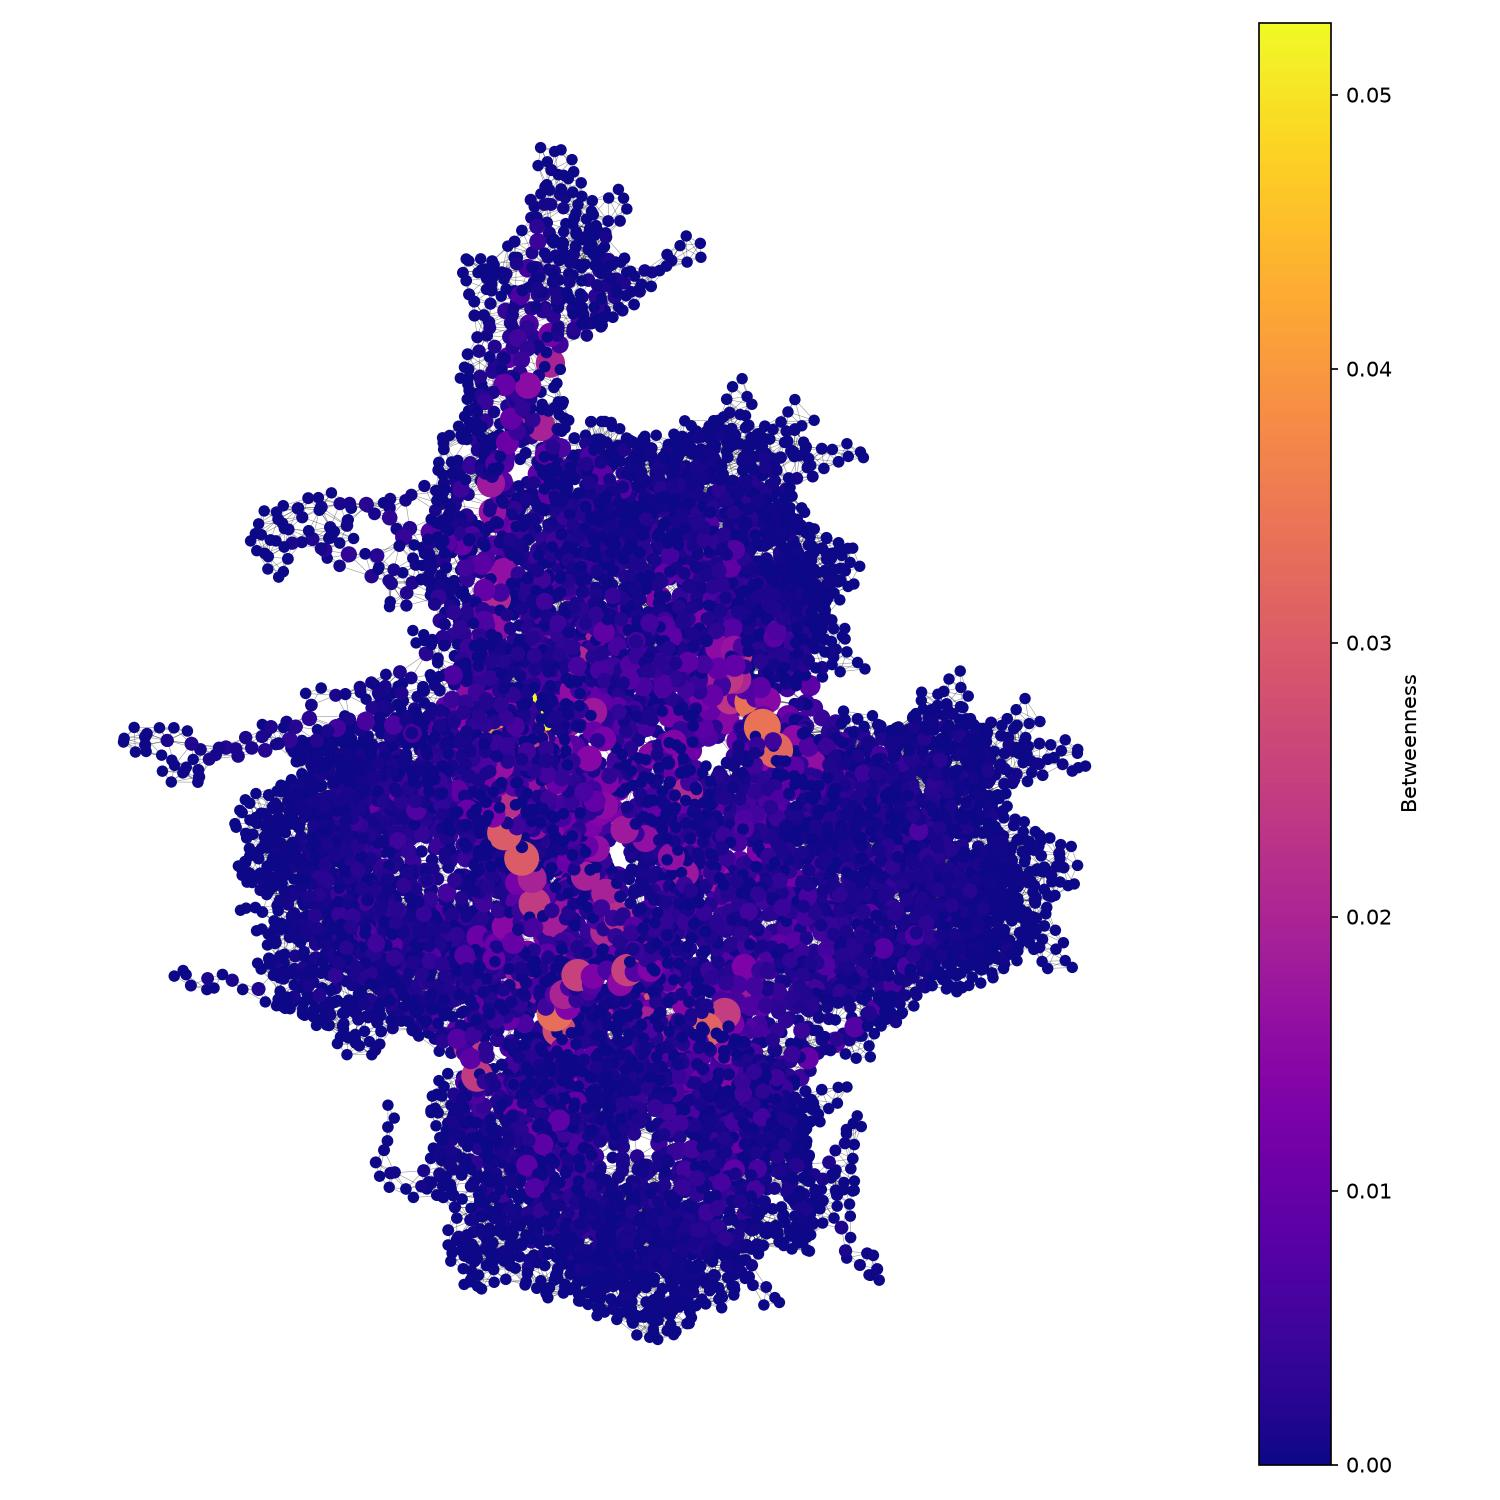
\includegraphics[width=0.7\textwidth]{figures/6B1T-contact-betweenness.jpg}
		\caption{Rede de contato do 6B1T projetada nas coordenadas da estrutura, com os nós coloridos pela centralidade de intermediação.}
		\label{fig_betw_6b1t}
	\end{figure}

	Em resumo, a topologia das redes de contato reflete a estrutura tridimensional da proteína. Isso pode indicar que a detecção de comunidades nesse tipo de rede será mais adequada para identificar grupos separados espacialmente, o que nem sempre ocorre com as famílias.

	\subsection{Detecção de comunidades nas redes de contato}
	\label{sec_varredura}

	Para validar esse modelo, foi criado um pipeline de varredura (\texttt{model\_selection}) que constrói cada rede com vários limiares, aplica diferentes algoritmos de detecção de comunidades (Louvain, Infomap, greedy modularity, label propagation e bipartição espectral) e compara cada partição obtida com as anotações por meio do índice ARI (\emph{Adjusted Rand Index}). O valor 1 indica uma partição idêntica à anotação, enquanto 0 indica equivalência a uma partição aleatória.

	Aplicando a varredura às três proteínas de teste, a configuração de rede de contato que maximizou o ARI em cada uma é apresentada na Tabela~\ref{tab_contato}.

	\begin{table}[H]
		\centering
		\caption{Melhor configuração de rede de contato por proteína de teste (máximo ARI na varredura).}
		\begin{tabular}{llrlrr}
			\toprule
			\textbf{Proteína (famílias)} & \textbf{Rede} & \textbf{Limiar} & \textbf{Algoritmo} & \textbf{Comunidades} & \textbf{ARI} \\
			\midrule
			4HHB ($\alpha$, $\beta$) & Resíduo & 6 Å & Infomap & 4 & 0,49 \\
			1AON (Cpn60, Cpn10) & Cadeia & 12 Å & Espectral & 2 & 1,00 \\
			6MID (poliproteína, anticorpo) & C$\alpha$ & 5 Å & Espectral & 2 & 0,47 \\
			\bottomrule
		\end{tabular}
		\label{tab_contato}
	\end{table}

	No geral, as redes de contato em nível atômico (C$\alpha$, C$\beta$, resíduo) identificam a organização geométrica, ou seja, as cadeias e as regiões que estão espacialmente separadas, e não as famílias.

	No 6MID, o resultado é apenas parcial: a rede separa a cadeia que está espacialmente isolada, mas não distingue duas famílias cujas cadeias estão espacialmente entrelaçadas, resultando em um ARI de 0,47 (Figura~\ref{fig_6mid}).

	\begin{figure}[H]
		\centering
		\begin{minipage}{0.48\textwidth}
			\centering
			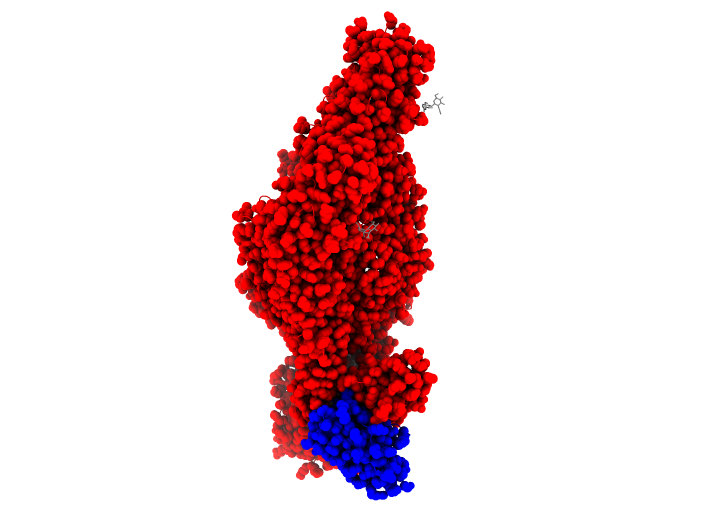
\includegraphics[width=\textwidth]{figures/6MID-chimerax-contact_comm.png}
		\end{minipage}\hfill
		\begin{minipage}{0.48\textwidth}
			\centering
			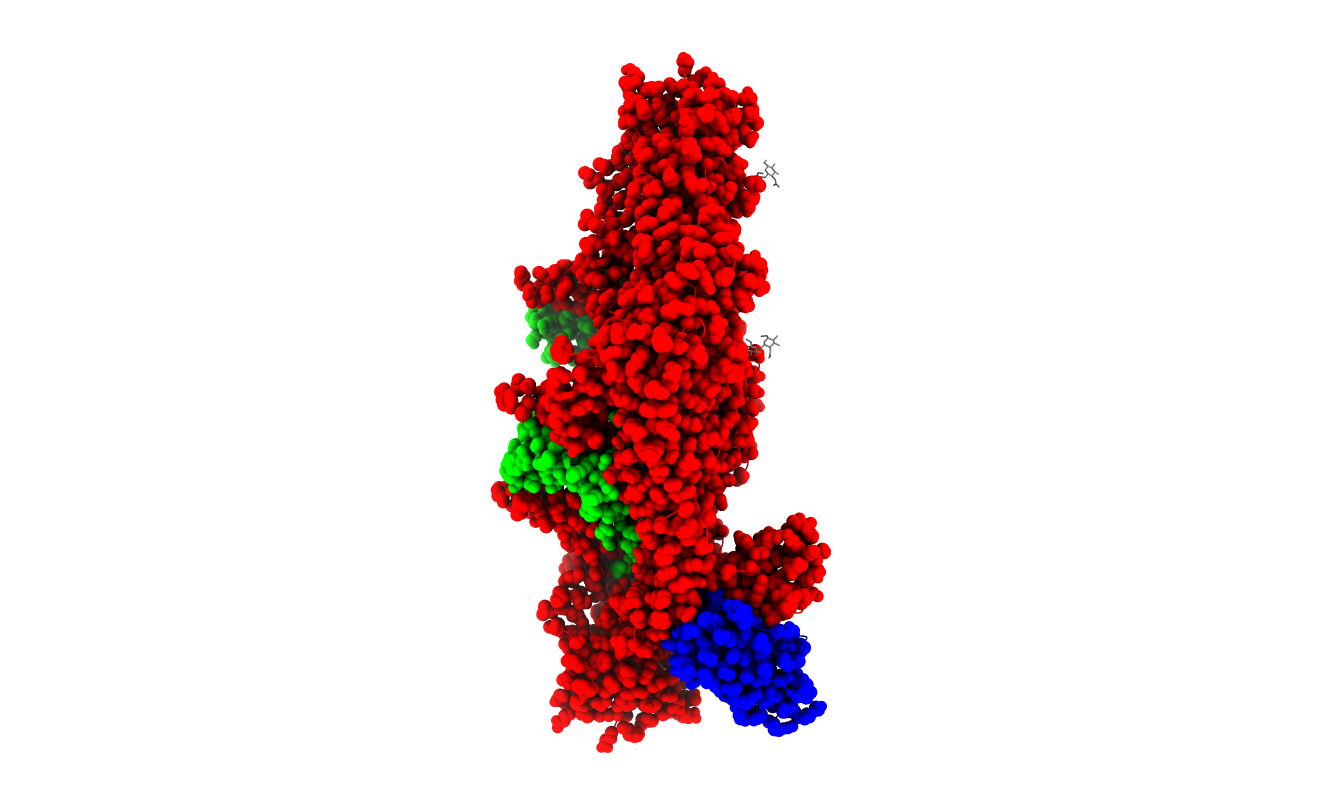
\includegraphics[width=\textwidth]{figures/6MID-chimerax-desired_comm.png}
		\end{minipage}
		\caption{6MID: à esquerda, a melhor divisão obtida pela rede de contato; à direita, as cadeias coloridas por família.}
		\label{fig_6mid}
	\end{figure}

	Já no 4HHB, em que as famílias $\alpha$ e $\beta$ se intercalam espacialmente, nenhuma rede de contato recupera a divisão $\alpha$/$\beta$, sendo o ``melhor'' resultado a separação das cadeias individuais (Figura~\ref{fig_4hhb}).

	\begin{figure}[H]
		\centering
		\begin{minipage}{0.48\textwidth}
			\centering
			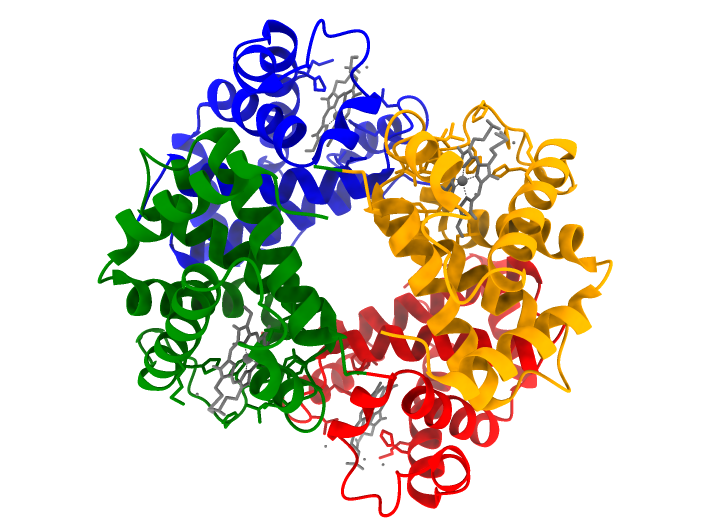
\includegraphics[width=\textwidth]{figures/4HHB-chimerax-contact_comm.png}
		\end{minipage}\hfill
		\begin{minipage}{0.48\textwidth}
			\centering
			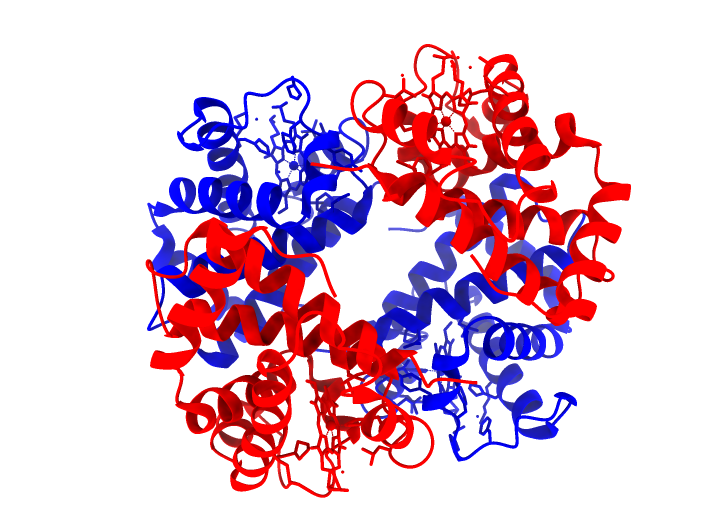
\includegraphics[width=\textwidth]{figures/4HHB-chimerax-desired_comm.png}
		\end{minipage}
		\caption{4HHB: à esquerda, a melhor divisão obtida pela rede de contato; à direita, as cadeias coloridas por família.}
		\label{fig_4hhb}
	\end{figure}

	A exceção é o 1AON. Como as cadeias de uma das famílias formam um bloco espacialmente distinto das cadeias da outra, a rede de contato de cadeias separa as duas famílias (ARI 1,00), como mostra a Figura~\ref{fig_1aon}.

	\begin{figure}[H]
		\centering
		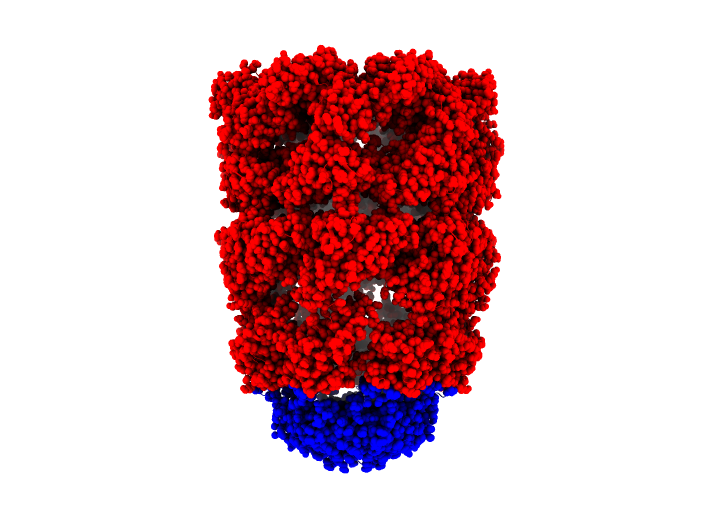
\includegraphics[width=0.6\textwidth]{figures/1AON-chimerax-comm.png}
		\caption{1AON colorido pelas comunidades da rede de contato de cadeias.}
		\label{fig_1aon}
	\end{figure}

	Em suma, a rede de contato identifica o que está espacialmente agrupado, o que só coincide com as famílias quando elas formam blocos espaciais distintos. O teste no alvo confirma esse limite: aplicando as redes de contato ao 6B1T, a melhor configuração (rede C$\alpha$, limiar de 4 Å e bipartição espectral) atingiu apenas ARI 0,33, dividindo o alvo em 26 comunidades, em vez das 8 famílias (Figura~\ref{fig_6b1t}).

	\begin{figure}[H]
		\centering
		\begin{minipage}{0.48\textwidth}
			\centering
			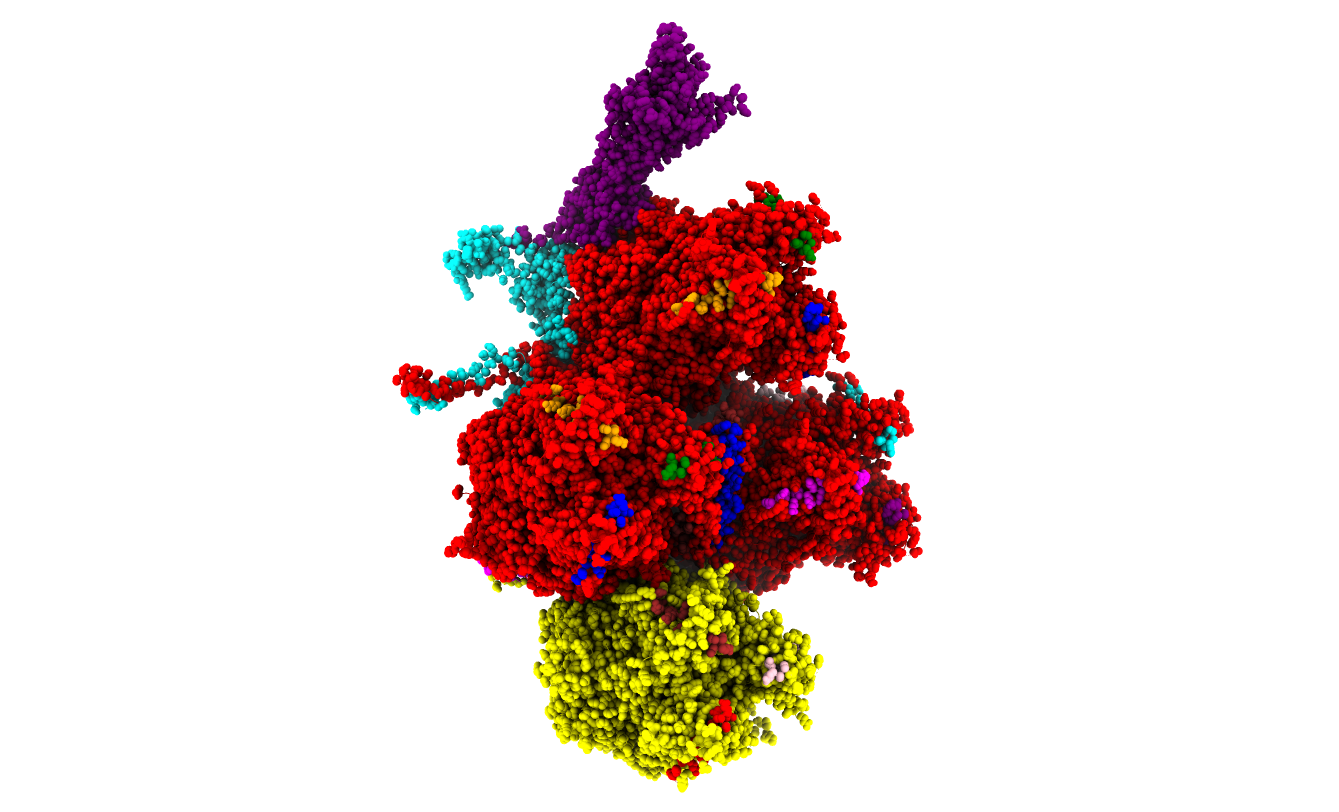
\includegraphics[width=\textwidth]{figures/6B1T-chimerax-contact_comm.png}
		\end{minipage}\hfill
		\begin{minipage}{0.48\textwidth}
			\centering
			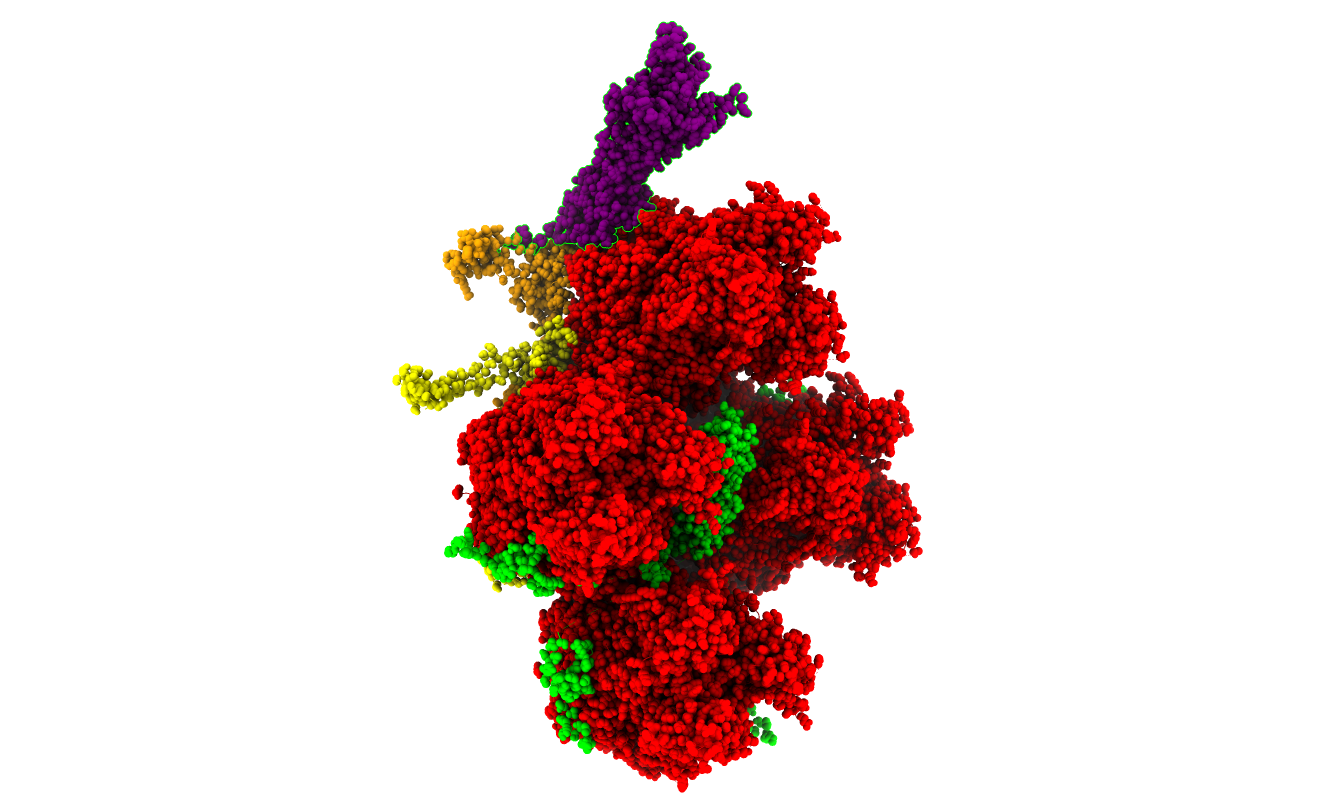
\includegraphics[width=\textwidth]{figures/6B1T-chimerax-desired_comm.png}
		\end{minipage}
		\caption{6B1T: à esquerda, as comunidades da rede de contato; à direita, as cadeias coloridas por família.}
		\label{fig_6b1t}
	\end{figure}

	\subsection{Rede de similaridade de cadeias}
	\label{sec_similaridade}

	Como as famílias são definidas pela identidade de sequência, isto é, cadeias da mesma proteína têm sequências de aminoácidos muito semelhantes, foi construída uma rede cujas arestas indicam diretamente essa semelhança:

	\begin{itemize}
		\item \textbf{Nó:} cada cadeia da estrutura;
		\item \textbf{Aresta:} liga duas cadeias cuja similaridade de sequência é maior ou igual a um limiar;
		\item \textbf{Peso:} a própria similaridade.
	\end{itemize}

	Dessa forma, cadeias da mesma proteína formam agrupamentos densos, e a detecção de comunidades nesse grafo tende a recuperar as famílias. A sequência de cada cadeia é obtida tomando-se um resíduo por posição e convertendo-se o código de três letras para o de uma letra, por exemplo, ALA e GLY em A e G.

	A similaridade entre duas cadeias é medida de duas formas:

	\begin{itemize}
		\item \textbf{Cosseno de $k$-mers (padrão).} Cada sequência é transformada em um vetor com a contagem de todos os seus $k$-mers (subcadeias de comprimento $k$; por padrão, $k = 3$), e a similaridade é o cosseno entre esses vetores. Trata-se de um método livre de alinhamento, com custo linear em relação ao comprimento da sequência e robusto à ausência de resíduos, que faria uma comparação por igualdade exata falhar.
		\item \textbf{Identidade por alinhamento.} Realiza-se um alinhamento global (Needleman--Wunsch, por meio do Biopython), contam-se as posições idênticas e normaliza-se o resultado pelo maior comprimento das duas sequências.
	\end{itemize}

	O limiar é um valor entre 0 e 1. Esse é o modelo adotado no restante do trabalho.

	\section{Detecção de comunidades na rede de similaridade}
	\label{sec_deteccao}

	A detecção de comunidades é, agora, aplicada à rede de similaridade, primeiro nas proteínas de teste e, depois, no alvo, com os mesmos cinco algoritmos e o mesmo protocolo de avaliação da Seção~\ref{sec_varredura}.

	\subsection{Testes preliminares}
	\label{sec_testes_sim}

	Repetindo a varredura sobre a rede de similaridade nas três proteínas de teste, obtêm-se os resultados da Tabela~\ref{tab_similaridade}.

	\begin{table}[H]
		\centering
		\caption{Melhor configuração da rede de similaridade por proteína de teste.}
		\begin{tabular}{lrlrr}
			\toprule
			\textbf{Proteína (famílias)} & \textbf{Limiar} & \textbf{Algoritmo} & \textbf{Comunidades} & \textbf{ARI} \\
			\midrule
			4HHB ($\alpha$, $\beta$) & 0,5 & Louvain & 2 & 1,00 \\
			1AON (Cpn60, Cpn10) & 0,5 & Louvain & 2 & 1,00 \\
			6MID (poliproteína, anticorpo) & 0,5 & Louvain & 4 & 1,00 \\
			\bottomrule
		\end{tabular}
		\label{tab_similaridade}
	\end{table}

	Para as três proteínas, o resultado obtido é a identificação exata das famílias anotadas (ARI 1,00), independentemente de sua disposição espacial, o que confirma a escolha do modelo apresentada na Seção~\ref{sec_similaridade}.

	\subsection{Alvo 6B1T}
	\label{sec_alvo}

	No alvo, a rede de similaridade se fragmenta em oito cliques, um por família, o que torna a detecção trivial. O grau de cada nó é igual ao tamanho de sua família menos um, o clustering é máximo dentro de cada clique, a assortatividade é perfeita e a intermediação é nula, pois não há nenhuma ponte entre as famílias. A Figura~\ref{fig_sim_graph} mostra essa estrutura de cliques.

	\begin{figure}[H]
		\centering
		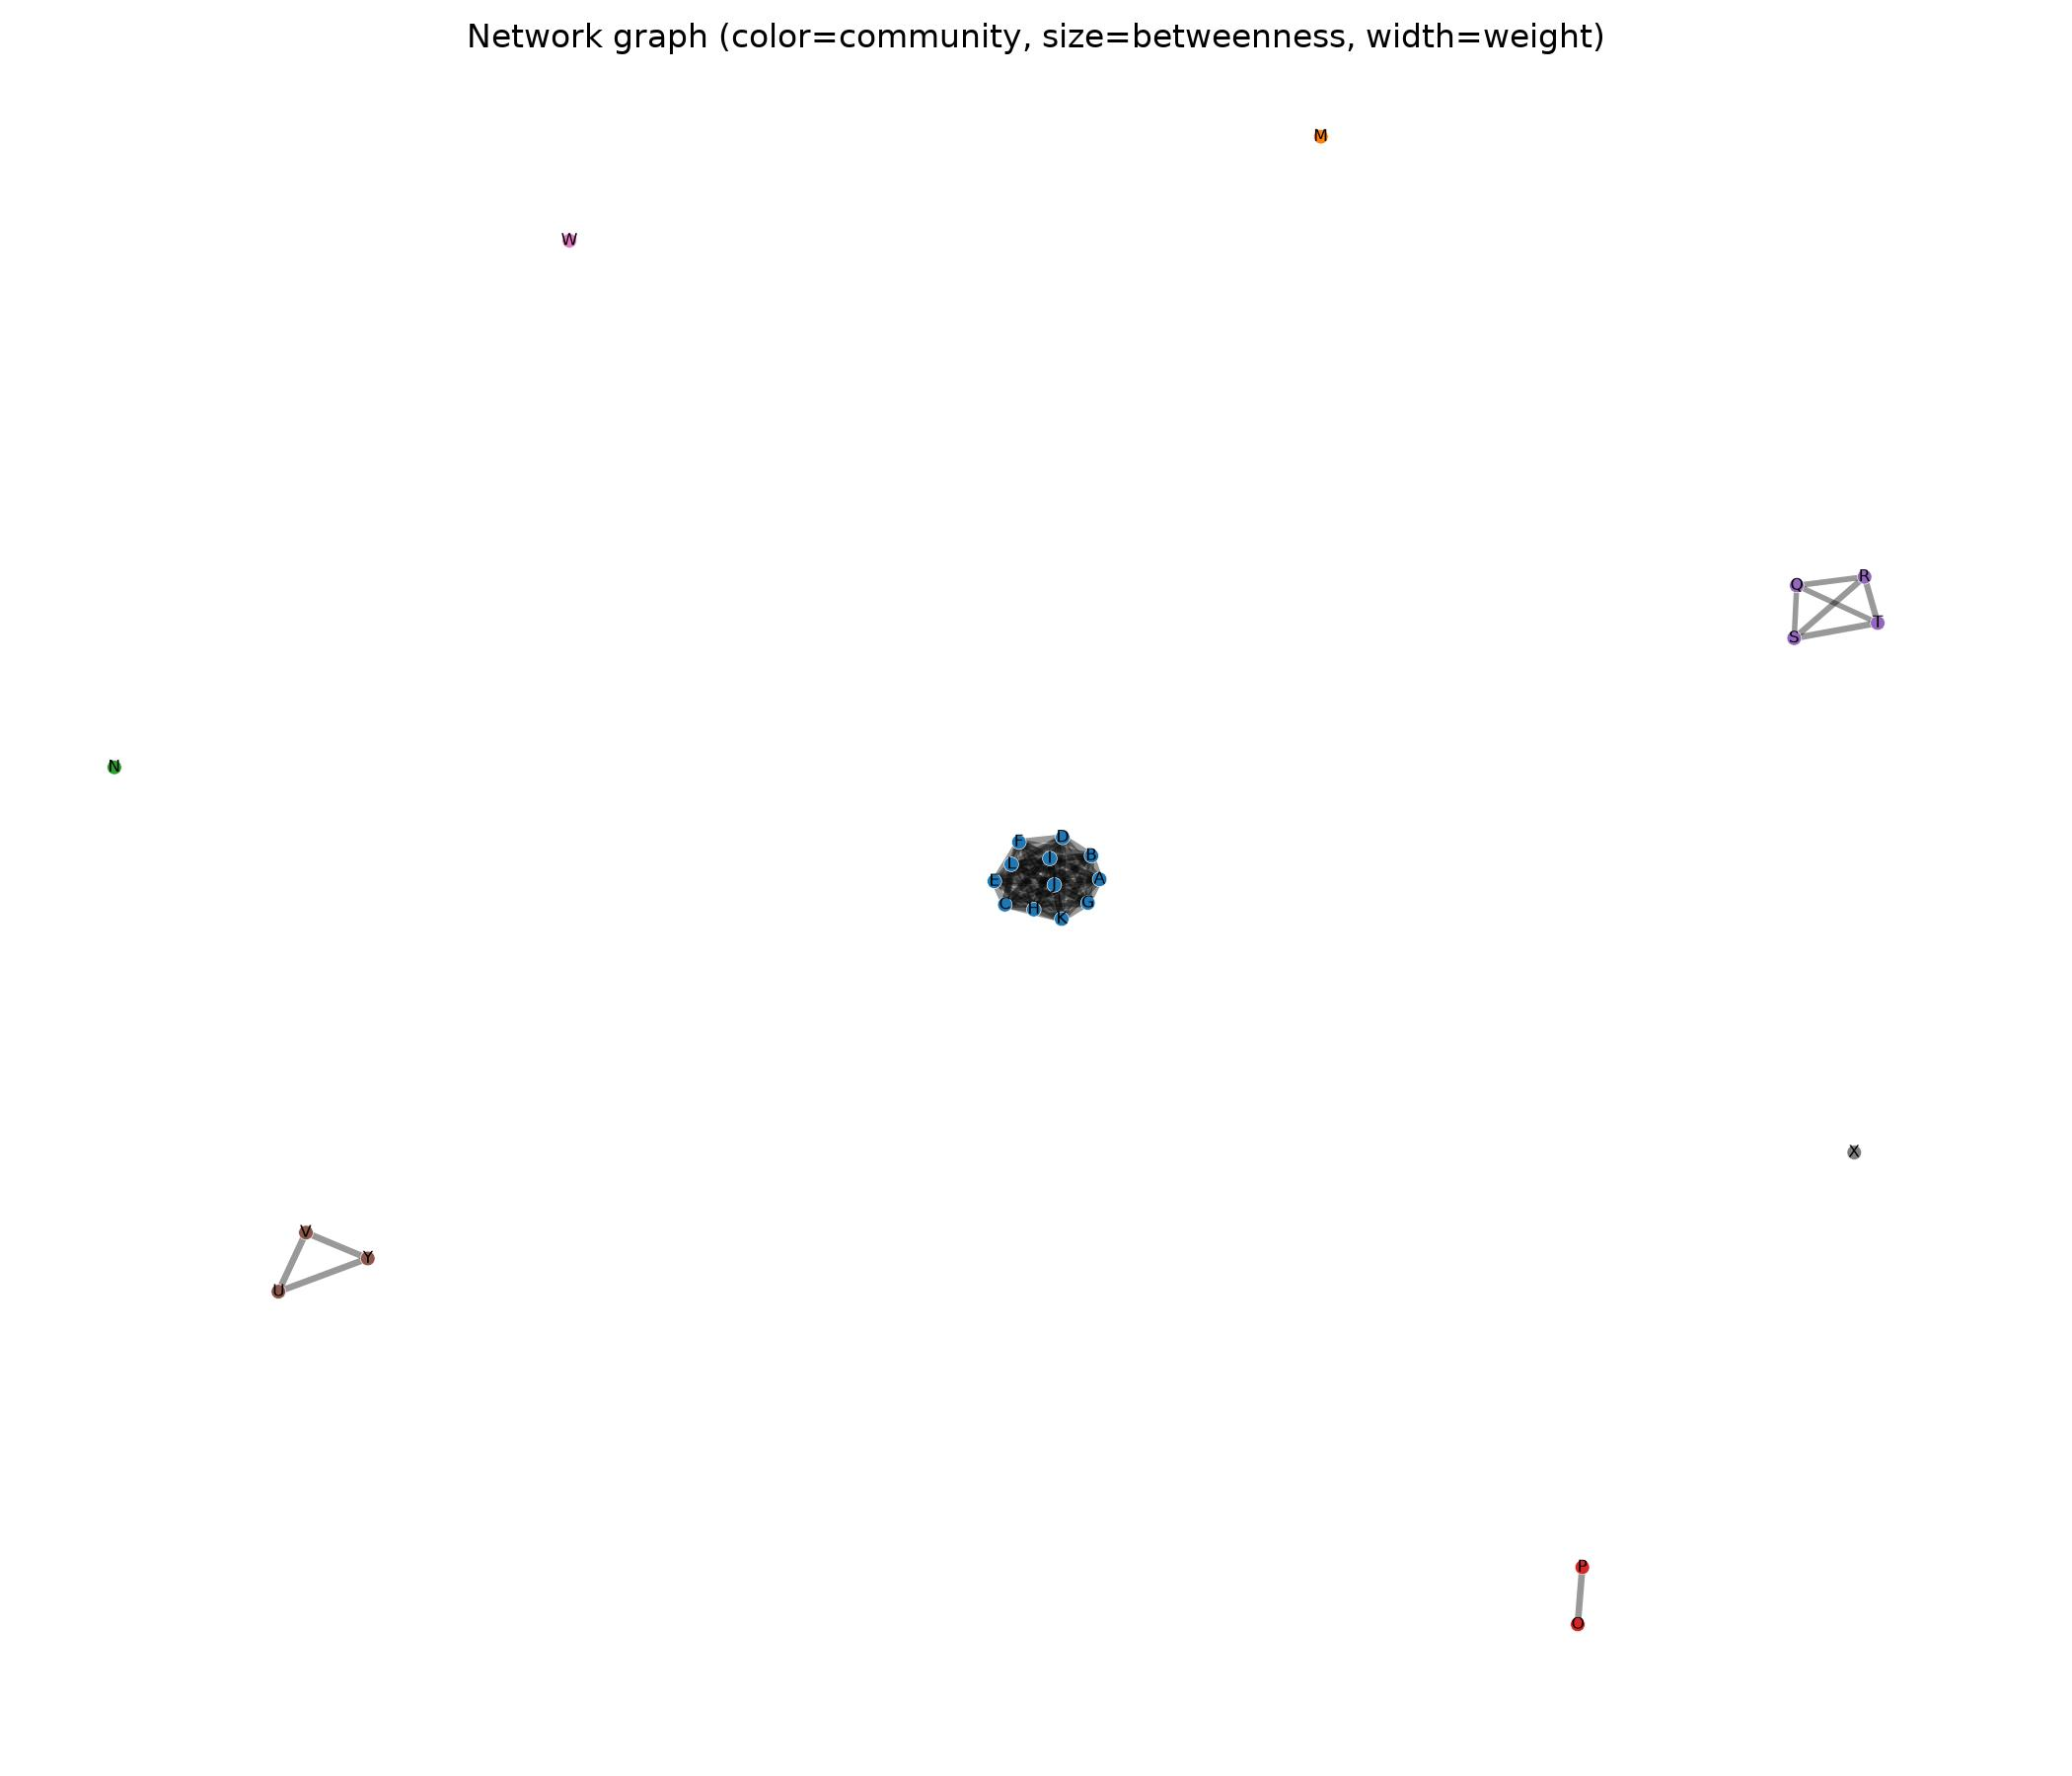
\includegraphics[width=0.7\textwidth]{figures/6B1T-sim-graph.jpg}
		\caption{Rede de similaridade de cadeias do 6B1T.}
		\label{fig_sim_graph}
	\end{figure}

	Como cada família já constitui um componente isolado, todos os algoritmos convergem para a mesma partição, recuperando os oito componentes como oito comunidades. A partição identifica exatamente as famílias anotadas, com ARI igual a 1,00. A Tabela~\ref{tab_contingencia} mostra a matriz de contingência entre comunidades e famílias. Por ser uma matriz diagonal, nenhuma comunidade mistura famílias, ou seja, cada comunidade corresponde exatamente a uma família.

	\begin{table}[H]
		\centering
		\caption{Matriz de contingência entre as comunidades detectadas e as famílias anotadas do 6B1T.}
		\begin{tabular}{lrrrrrrrr}
			\toprule
			\textbf{Família} & \textbf{C1} & \textbf{C2} & \textbf{C3} & \textbf{C4} & \textbf{C5} & \textbf{C6} & \textbf{C7} & \textbf{C8} \\
			\midrule
			hexon  & 12 & 0 & 0 & 0 & 0 & 0 & 0 & 0 \\
			IX     & 0  & 4 & 0 & 0 & 0 & 0 & 0 & 0 \\
			VI     & 0  & 0 & 3 & 0 & 0 & 0 & 0 & 0 \\
			VIII   & 0  & 0 & 0 & 2 & 0 & 0 & 0 & 0 \\
			penton & 0  & 0 & 0 & 0 & 1 & 0 & 0 & 0 \\
			IIIa   & 0  & 0 & 0 & 0 & 0 & 1 & 0 & 0 \\
			VII    & 0  & 0 & 0 & 0 & 0 & 0 & 1 & 0 \\
			VI\textsubscript{2} & 0 & 0 & 0 & 0 & 0 & 0 & 0 & 1 \\
			\bottomrule
		\end{tabular}
		\label{tab_contingencia}
	\end{table}

	A Figura~\ref{fig_sim_3d} projeta as comunidades detectadas sobre as coordenadas da estrutura, colorindo cada cadeia de acordo com a comunidade à qual pertence. Como as comunidades coincidem com as famílias, essa projeção é idêntica à coloração por família da Figura~\ref{fig_6b1t}, confirmando visualmente a recuperação.

	\begin{figure}[H]
		\centering
		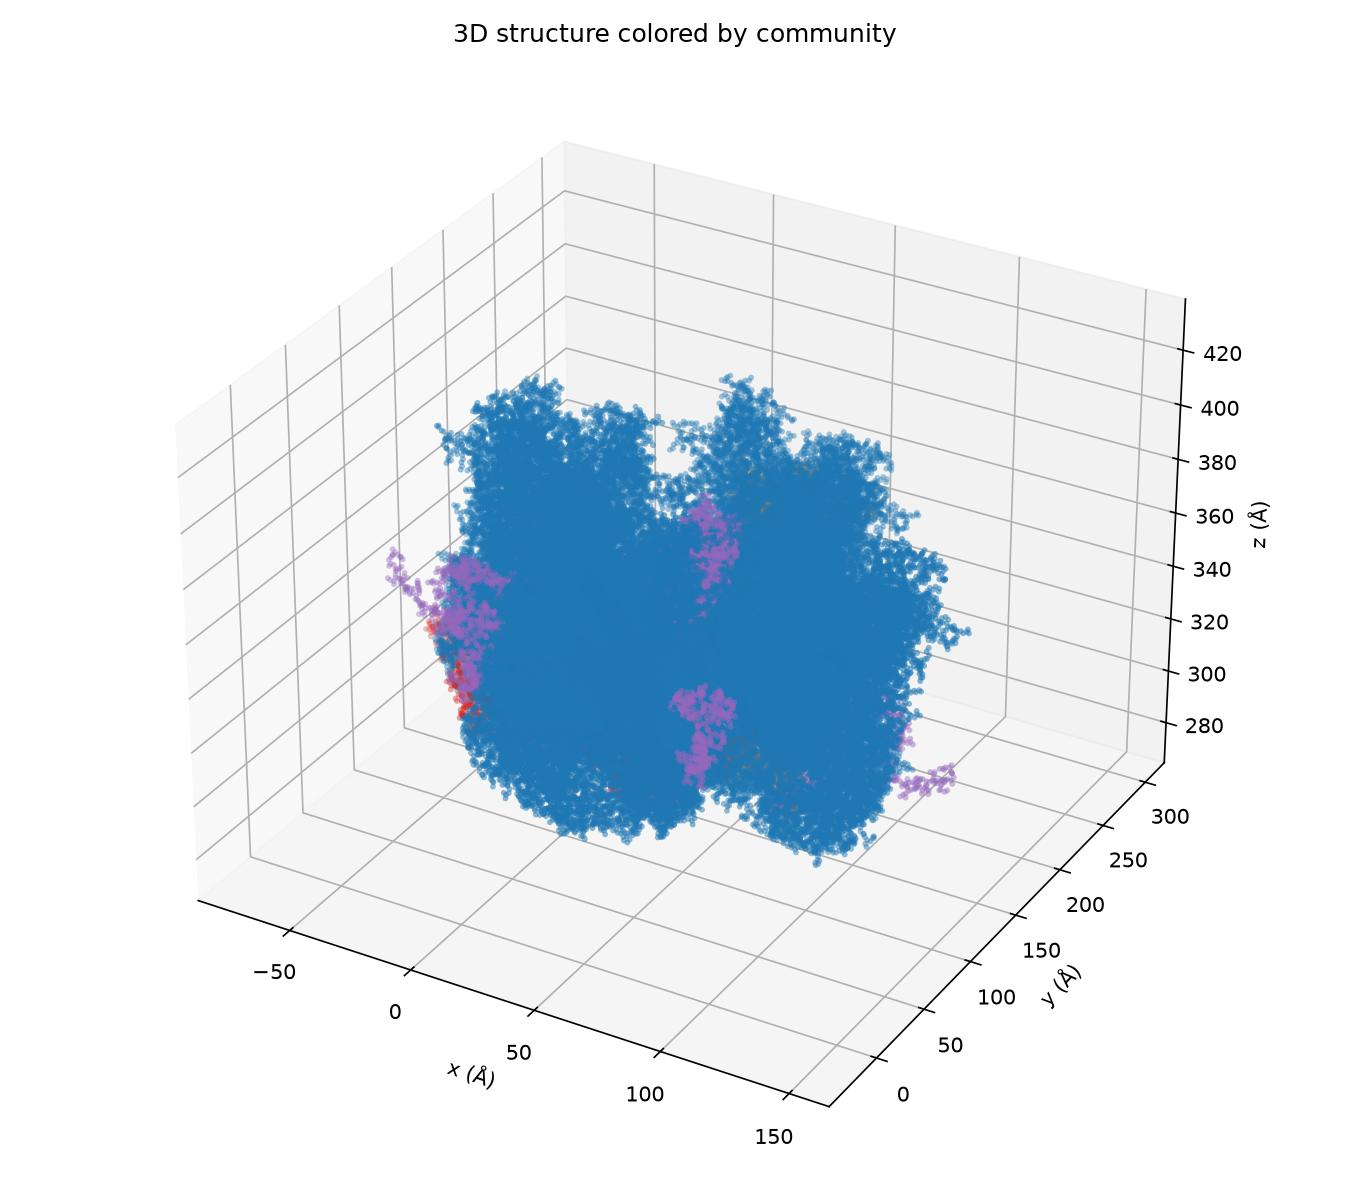
\includegraphics[width=0.7\textwidth]{figures/6B1T-sim-structure_3d.jpg}
		\caption{Comunidades detectadas na rede de similaridade, projetadas sobre as coordenadas da estrutura do 6B1T; cada cadeia é colorida de acordo com sua comunidade.}
		\label{fig_sim_3d}
	\end{figure}

	\section{Conclusão}
	\label{sec_conclusao}

	Este trabalho investigou se a detecção de comunidades no grafo de uma proteína recupera suas famílias anotadas. A conclusão central é que a resposta depende da modelagem das arestas. Nas redes de contato, cujas arestas ligam elementos espacialmente próximos, a topologia reflete a estrutura tridimensional, e as comunidades acompanham a geometria, não as famílias. Já na rede de similaridade de cadeias, cujas arestas ligam cadeias com sequências semelhantes, cada família forma um componente denso e desconexo, e a detecção de comunidades recupera diretamente essas famílias.

	No alvo 6B1T, a melhor configuração de rede de contato atingiu apenas ARI 0,33, fragmentando a estrutura em comunidades geométricas, enquanto a rede de similaridade recuperou as oito famílias. O mesmo padrão se repetiu nas três proteínas de teste.

	\bibliographystyle{apalike-pt}
	\bibliography{references}

\end{document}
